\documentclass{article}
\usepackage[margin=1in]{geometry}
\usepackage{tabulary}
\usepackage{float}
\usepackage{lipsum}
\usepackage[utf8]{inputenc}
\usepackage{hyperref}
\usepackage{graphicx}
\usepackage{graphics}
\usepackage{listings}
\lstset
{ %Formatting for code in appendix
    language=C,
    basicstyle=\small,
    numbers=left,
    stepnumber=1,
    showstringspaces=false,
    tabsize=1,
    breaklines=true,
    breakatwhitespace=false,
}
\usepackage{xcolor}
\lstset{escapeinside={<@}{@>}}
\usepackage[T1]{fontenc}
\usepackage[parfill]{parskip}
\newcommand{\code}[1]{\textsf{#1}}
\setlength{\parindent}{0em}
\begin{document}
\begin{center}{\LARGE ECE 264: Advanced C Programming} \end{center}
\begin{center}{\large Programming Assignment 9 - Expression Trees, Due 7/31/19} \end{center}

\bigskip
{\em This assignment is a bonus assignment. This is extra credit (it has the same weight as all other assignments)}

This assignment is the second in a two-part series on building a calculator. It follows on from PA08, but does not directly build on it (you do not need a working PA08 to successfully complete this assignment). In PA08, you had to build an RPN calculator that took a postfix expression and computed the result. In this assignment, you will build a tool that converts an {\em infix} expression (i.e., an expression that looks `normal'') into a postfix output that the PA08 calculator can operate on.


This assignment essentially asks you to write a very basic compiler. We provide some additional background about compilers in note boxes (like this one) throughout the background section, but you can ignore them if you want. If you're interested in learning more about how compilers work, take ECE 468.


\section{Learning Goals}
In this assignment, you will learn

\begin{enumerate}
\item    Basic expression parsing
\item    Building a tree bottom-up
\item    Performing a post-order traversal of a tree
\end{enumerate}

\section{Background}

\subsection{Fully parenthesized infix expressions}

Infix expressions are the `normal'' way you're used to seeing arithmetic expressions written out (e.g., \textsf{2 + 3 * 7}), with all the complications of order-of-operations, etc. We will use a simpler version of infix expressions that we will call `fully parenthesized'': every binary operation is enclosed in parentheses. So \textsf{2 + 3 * 7} would be written \textsf{(2 + (3 * 7))}. Note that because we put parentheses everywhere, we can ignore order of operations.


To precisely capture what a fully parenthesized expression is, we can define a fully parenthesized infix expression {\em recursively}. A fully parenthesized expression is:

\begin{enumerate}
\item A (floating point) number
\item An open parenthesis `(' followed by a {\em fully parenthesized expression} (which also follows these rules) followed by an operator (\textsf{+, -, *,} or \textsf{ \ } ) followed by another {\em fully parenthesized expression} followed by a closed parenthesis `)'.
\end{enumerate}

Defining expressions and other things recursively is very common in computer science/engineering, so people have come up with notation to directly capture the recursive rules laid out above. We would express these rules as:

\begin{enumerate}
\item        \textsf{E -> lit}
\item        \textsf{E -> (E op E)}
\end{enumerate}

\subsection{Basic expression parsing}

The process of determining whether a string is a valid fully-parenthesized expression and breaking that expression into its components (`this is a number'', `this is a parenthesized sub-expression'', etc.) is called {\em parsing}. The way to do this is to look at the rules that define a valid fully-parenthesized expression and decide whether a given string obeys those rules (i.e., you could use those rules to generate the string).


There is a whole sub-field of computer science devoted to determining how to parse strings (in fact, a parser is one of the major components of a compiler: it determines what parts of your code are if statements, what parts are variable declarations, etc.). But our rules for fully-parenthesized expressions are simple enough that we can write a simple recursive function to decide whether an expression is valid.

\subsection{Tokenization}
The first step in parsing is to {\em tokenize} a string: to turn a string of characters into a string of "words" that represent the individual pieces of an expression. We call these words {\em tokens}. In other words, a tokenizer's job is to take a string like:


\textsf{(3 + (7 * 8))}


And tell you the individual words (tokens) in the string:


\textsf{LPAREN VAL ADD LPAREN VAL MUL VAL RPAREN RPAREN}


In this case, \textsf{LPAREN} means the character \textsf{(}, \textsf{VAL} means any number, \textsf{RPAREN} means the character \textsf{)}, and \textsf{ADD} and \textsf{MUL} are (hopefully) self-explanatory.


    It might seem like adding an extra step to turn a fairly simple expression into a bunch of tokens, but this is useful because that way later stages of parsing don't have to worry about things like skipping over white space, or deciding whether \textsf{8))} is one word or three (in this case, it's three!).


The tool that tokenizes a string is called a {\em tokenizer} or a {\em scanner}. We have written a scanner for you (in \textsf{scanner.c}) that reads in a file, breaks it up into tokens, and lets you find the next token in the string by calling \textsf{nextToken}. Pay close attention to the \textsf{Token} data type defined in \textsf{scanner.h}!

\subsection{Recursive parsing}
Given a tokenizer, we can now write a simple recursive function to tell whether a string is a valid, fully-parenthesized expression. Here is the algorithm, which you can wrap in a function that returns a \textsf{bool}.

\begin{enumerate}
\item    Get the next token
\item    If the next token is a \textsf{VAL} (matches rule 1), this is a valid fully-parenthesized expression. Return \textsf{true}.
\item    If the next token is an \textsf{LPAREN} we now try to match all of rule 2:
\begin{enumerate}
\item        We have already seen the \textsf{LPAREN}, so the next thing we expect to see is a fully-parenthesized expression. We can just call {\em this same function} recursively to do that! If the recursive call returns \textsf{true}, it means we have found a fully-parenthesized expression
\item        The next part of rule 2 is to match an operation, so we grab the next token and see if it is an \textsf{ADD, SUB, MUL,} or \textsf{DIV}. If it is, we continue.
\item        Then we call this same function recursively again to find another fully-parenthesized expression.
\item        Finally, we grab the next token to see if it is an \textsf{RPAREN}. If it is, we have matched rule 2, and this is a fully-parenthesized expression, so we return \textsf{true}.
\end{enumerate}
\end{enumerate}

If any of those steps fail, that means we don't see what we expect, and the string is not a fully-parenthesized expression, so we should return \textsf{false}.


    The recursive function we wrote is a simplified version of a {\em recursive descent parser}. These types of parsers are not quite powerful enough to decide, for example, if a given program is a valid C program (the rules for valid C programs are too complicated). But they're still pretty powerful.

\subsection{Expression trees}

A useful way to represent a fully-parenthesized expression is using an {\em expression tree}. This is a binary tree where each {\em leaf node} (node with no children) is a number, and each {\em interior node} (a node with two children) is an arithmetic operation. The structure of the expression tree matches the parentheses: each fully-parenthesized (sub) expression becomes its own (sub) tree. So, for example, \textsf{(7 + (8 * 10))} has an expression tree that looks like:

\begin{figure}[H]
\centering
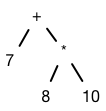
\includegraphics[scale=0.5]{exptree1.png}
\end{figure}

While a more complicated expression like: ((7 + (8 * 10)) - (2 + 3)) has an expression tree that looks like:

\begin{figure}[H]
\centering
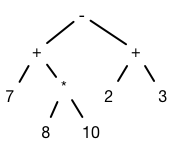
\includegraphics[scale=0.5]{exptree2.png}
\end{figure}

(Note that the expression (7 + (8 * 10)) appears as a subexpression here, so its expression tree appears as the left subtree in the larger tree.)

\subsection{Building expression trees}

Interestingly, you can {\em build} an expression tree from a fully-parenthesized expression during the process of parsing it (using the recursive approach from above). The key is the concept of building a tree `bottom up''.


In class, we have seen how to build trees `top down'' (think binary search trees): we start by creating the root, then we add new nodes by adding children to nodes at the `bottom'' of the tree. The tree `grows'' from the top down: we create a node before we create any of its descendants.


The idea behind {\em bottom up} tree construction is that we create a tree by {\em first} creating the subtrees, then making those subtrees the left and right children of a newly-created root. In other words, we create a node by first creating its descendants.


We can modify our recursive parser from above to build trees instead. The idea is that invoking the parser function returns an expression tree that represents the (sub)expression we just matched. Rather than returning a \textsf{bool}, we can have it return a \textsf{TreeNode *}.

\begin{itemize}
\item    In step 1, where we used to return \textsf{true} because we found a value, we can instead return a pointer to a newly-allocated \textsf{TreeNode} containing that value. (This \textsf{TreeNode} doesn't need left or right children -- recall that in values are the leaves of an expression tree.).
\item    In step 2, each of the recursive calls to the parse function will return \textsf{TreeNode *} pointers to trees that represent the sub-expression we matched. These can become the left and right children of a new node, whose value is the {\em operator} we match in step 2. This new node can be returned as the root of a tree representing the expression we just matched.
\end{itemize}

\subsection{Example}

So let's see how our parse function would work for \textsf{(7 + (8 * 10))}:
\begin{itemize}
\item    We start by seeing an \textsf{LPAREN}, so we're trying to match rule 2.
\item    We invoke the recursive method again.
\begin{itemize}
\item    We see a VAL, so we build a node containing that value, and return it:
	
	\textsf{7}

\end{itemize}
\item We see an \textsf{ADD}, which we remember, but don't do anything with
\item We invoke the recursive method again.
\begin{itemize}
\item  We see an \textsf{LPAREN}, so we're trying to match rule 2.
\item  We invoke the recursive method again.
\begin{itemize}
\item  We see a \textsf{VAL}, so we build a node containing that value and return it:


8


\end{itemize}
\item We see a \textsf{MUL}, which we remember, but don't do anything with
\item We invoke the recursive method again.
\begin{itemize}
\item  We see a \textsf{VAL}, so we build a node containing that value and return it:
	

10


\end{itemize}
\item We create a new \textsf{TreeNode} storing the \textsf{MUL}, and make its left and right children the \textsf{TreeNode}s we returned from the two recursive invocations:

\begin{figure}[H]
\centering
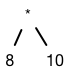
\includegraphics[scale=0.5]{step4.png}
\end{figure}

\item We see an \textsf{RPAREN}, so we return the new tree.
\end{itemize}

\item We create a new \textsf{TreeNode} storing the \textsf{ADD}, and make its left and right children the \textsf{TreeNode}s we returned from the two recursive invocations:
\begin{figure}[H]
\centering
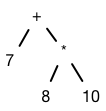
\includegraphics[scale=0.5]{step5.png}
\end{figure}

\item We see an \textsf{RPAREN}, so we return the new tree
\end{itemize}

\subsection{Postfix traversal}

There are three `standard'' ways to traverse a binary tree, each of which describes a way of recursively visiting each node of the tree.

\begin{enumerate}
\item    {\em inorder} recursively visits the left child, then processes the current node, then recursively visits the right child.
\item    {\em preorder} processes the current node, then recursively visits the left child, then recursively visits the right child.
\item    {\em postorder} recursively visits the right child, recursively visits the left child, then processes the current node.
\end{enumerate}

If `processing'' a node prints out its value, note that doing an {\em inorder} traversal of the expression tree recovers the original infix expression (though without the parentheses, so the order of operations might be screwy). If we print this expression tree inorder:

\begin{figure}[H]
\centering
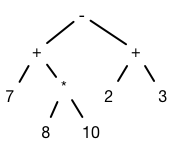
\includegraphics[scale=0.5]{exptree2.png}
\end{figure}

We get \textsf{7 + 8 * 10 - 2 + 3}, which looks like its source expression if you remove all the parentheses.


Printing the tree {\em preorder} instead gives us: \textsf{- + 7 * 8 10 + 2 3}.


Finally, printing the tree {\em postorder} give us: \textsf{7 8 10 * + 2 3 + -}.

Note that {\em this is exactly what the postfix representation of the source expression would be}. If we create an expression tree from a fully-parenthesized expression, {\em we can turn it into postfix by performing a postorder print!}

\section{What you have to do}

Your job is to:
\begin{enumerate}
\item    Write a recursive function to parse a fully-parenthesized infix expression and produce an expression tree
\item    Write a function to traverse the expression tree in postorder and print the postfix representation of the input expression to a file.
\end{enumerate}


We have given you many starter files:
\begin{enumerate}
\item    \textsf{tree.h} and \textsf{tree.c}: data structure definitions for \textsf{TreeNode}s, as well as basic allocation and deallocation routines. You may find the \textsf{printTree} routine useful for debugging.
\item    \textsf{scanner.h} and \textsf{scanner.c}: a scanner that reads in a fully-parenthesized expression from a file and creates a stream of tokens. You can invoke \textsf{nextToken} to get the next token from the input expression (the token definitions are in \textsf{scanner.h}). You may find the \textsf{printToken} routine useful for debugging.
\item    \textsf{expressionTree.h}: a header file containing two function declarations: one to build an expression tree, the other to print it out in postorder to a file.
\item    \textsf{pa09.c}: a driver file for the assignment, containing the main function.
\end{enumerate}


Your job is to write \textsf{expressionTree.c}, which contains two functions:


\begin{enumerate}
\item  \textsf{buildExpressionTree}: this is the recursive parsing function, which returns the root of an expression tree built from the input expression. The function takes a \textsf{Scanner} as an argument, which can be used to step through the tokens in the input expression.
\item    \textsf{makePostfix}: this function performs a post-order traversal of the expression tree (whose root is passed in as \textsf{t}) and writes it out to the file (whose \textsf{FILE} pointer is passed in as \textsf{fptr}). The output file should be an RPN expression that you can pass in to your calculator from PA08.
\end{enumerate}

{\em Do not modify any files other than \textsf{expressionTree.c!}}

\section{What you have to turn in}

Turn in only \textsf{expressionTree.c}. If you submit any other files, we will not use them: we will overwrite them with our own versions of those files during the grading process. Any helper methods you need should just be declared and defined directly within \textsf{expressionTree.c} (not in \textsf{expressionTree.h}).


\end{document}
